\chapter{Experiments}\label{chapter:experiments}

In this chapter, we study and experiment with the training method we introduced
in Chapter~\ref{chapter:training_method}. While the main goal is to outperform
both teacher models and the base student checkpoint, we also want to show that
each teacher contributes to the student's performance.

This chapter is laid out as follows. We describe the training data in
Section~\ref{section:val_training_data}. Next, we discuss how we compare models
in Section~\ref{section:validation_tasks} and present the student's
configuration and define the baselines in
Section~\ref{section:student_model_config_baselines}. Then we experiment with
the structural loss in Section~\ref{section:structural_loss}. With the
structural loss already given, we find the best performing contextual loss and
the weighting of the two losses in Section~\ref{section:structural_and_contextual}.
Finally, we summarize our experiments and findings in
Section~\ref{section:experiments_summary}.

\section{Training data}\label{section:val_training_data}

We create the training dataset for our validation, labelled as
\Dataset{val-500k}, similarly to how we put together the final training
dataset \Dataset{train-1M} in Chapter~\ref{chapter:evaluation}. In short,
we equally sample documents from English Wikipedia and RealNews articles
\citep{zellers2019defending}, which are at least 1200 Longformer tokens long.
We use a subset of Longformer's training data, to make the comparison between a
trained student model and its base checkpoint fair. In this way, the trained
student model will not see any new data compared to Longformer. Thus any
performance gains of the student model over its base checkpoint, can be
attributed to our training method, rather than to a higher-quality training
dataset.

We present \Dataset{val-500k}'s statistics in
Table~\ref{table:val_data_stats}. Very similar to \Dataset{train-1M},
\Dataset{val-500k} contains long documents that are, on average, over 1300
tokens long. Consequently only about 34\% of the documents could be processed
whole using a traditional Transformer such as RoBERTa \citep{liu2019roberta} or
SBERT. We also display document's length distribution in
Figure~\ref{fig:val_data_dist}. As Wikipedia contains relatively short
documents, while RealNews does not contain document shorter than 1200 tokens,
the source's distributions are well spaced out.


\begin{table}
  \centering
  \footnotesize

  \begin{tabular}{lrr}
    \toprule
      Split & Train & Validation \\
    \midrule
      Documents & 500 000 & 10 000 \\
      Tokens & 6.85e+08 & 1.37e+07 \\
      Tokens per document & 1370.74$\pm$1723.38 & 1371.65$\pm$1717.24 \\
      SBERT tokens over 384 & 70.56\% & 70.07\% \\
      SBERT tokens over 512 & 66.37\% & 66.14\% \\
    \bottomrule
  \end{tabular}

  \caption{Statistics of \Dataset{val-500k}. Apart from document count, token
  count and mean token count per document, we also show percentage of documents
  with the number of SBERT tokens above given threshold.}

  \label{table:val_data_stats}

\end{table}

\begin{figure}

  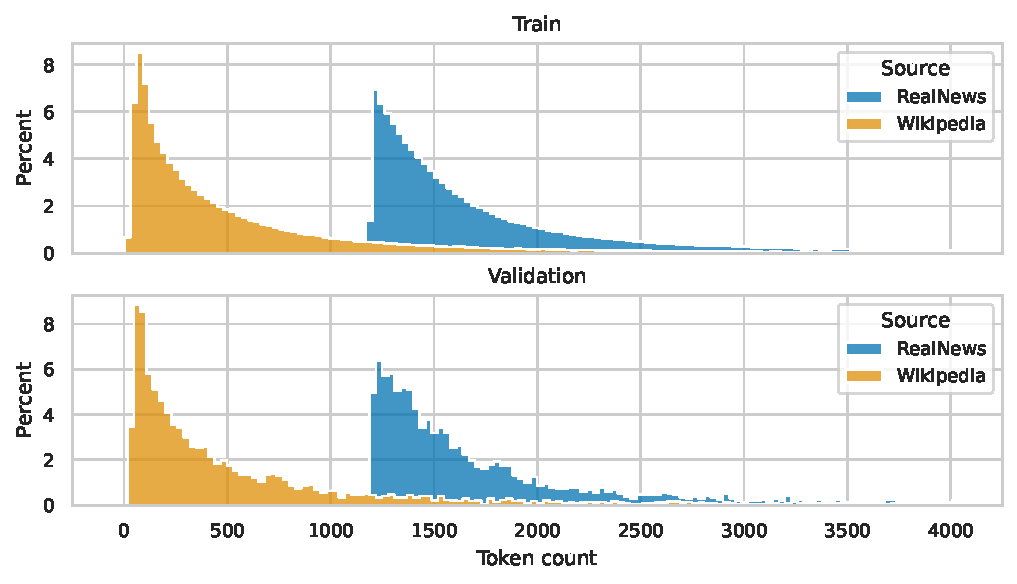
\includegraphics[width=\textwidth]{./img/val_data_dist.pdf}

  \caption{Distribution of train and validation documents' lengths for
  \Dataset{val-500k}.}

  \label{fig:val_data_dist}

\end{figure}

\section{Validation tasks}\label{section:validation_tasks}

We compare the embedding models based on their performance on a set of
downstream tasks. We use a subset of our evaluation tasks, which we describe in
detail in Chapter~\ref{chapter:evaluation}. We include tasks that have either
large enough training split suitable for cross-validation or a validation
split. All tasks are classifications that are evaluated using a validation
split, except for \Task{IMDB}, where we take the mean score of five
cross-validation folds. To make the validation faster to compute, we downsample
the validation and train splits to 10000 examples. We downsample the datasets
according to their label distribution, so that the truncated split has nearly
identical label distribution to the original one. We present the validation
tasks along with their document count in Table~\ref{table:validation_tasks}.

We use binary or micro-averaged accuracy as the scoring metric. Often we need
to compare performance across several tasks. However not all tasks are equally
difficult and so averaging accuracies would lead us to favoring models that
performed well on easy tasks, and undervaluing models that performed well on
the more difficult tasks. Therefore, we normalize the accuracy by the highest
score reached for the given task within the considered models and thereby
making the tasks equally difficult. We call this metric \emph{normalized
accuracy}. When more tasks taken into an account, we asses models based on the
mean normalized accuracy. In visualizations we mark mean normalized accuracy
with a black triangle.

When validating a trained embedding model on a task we finetune a head that
transforms the embeddings into the output format required by the given task. We
do not finetune the embedding model itself. Besides speeding up the validation,
this also gives us a more genuine picture of the embedding model's performance.
Since all our validation tasks are classifications, the heads are just 2-layer
neural network classifiers with a cross-entropy loss. We present the complete
list of classifier's hyperparameters and training parameters in
Table~\ref{table:head_train_params}.

\begin{table}
  \footnotesize
  \centering
  \begin{tabular}{llrrrr}
    \toprule
      & \multicolumn{2}{c}{Documents} & Classes & \multicolumn{2}{c}{Class percentage} \\
    \cline{2-3} \cline{5-6}
      Dataset & Train & Validation & & Train & Validation \\
    \midrule
      \Task{arxiv} \citep{arxiv_papers} & \dag10 000 & 2 500 & 11 & 9.09$\pm$1.24\% & 9.09$\pm$1.01\% \\
      \Task{imdb} \citep{maas2011learning} & \dag10 000 & - & 2 & 50.00$\pm$0.00\% & - \\
      \Task{oc} \citep{zhou2020multilevel} & \dag10 000 & \dag10 000 & 2 & 50.00$\pm$0.06\% & 50.00$\pm$0.15\% \\
      \Task{aan} \citep{zhou2020multilevel} & \dag10 000 & \dag10 000 & 2 & 50.00$\pm$1.50\% & 50.00$\pm$4.57\% \\
      \Task{s2orc} \citep{zhou2020multilevel} & \dag10 000 & \dag10 000 & 2 & 50.00$\pm$0.09\% & 50.00$\pm$0.32\% \\
      \Task{pan} \citep{zhou2020multilevel} & \dag10 000 & 2 908 & 2 & 50.00$\pm$0.00\% & 50.00$\pm$0.00\% \\
    \bottomrule
  \end{tabular}

  \caption{Validation tasks we use to compare embedding models, in this
  chapter. We truncated splits marked with {\dag} to speed up evaluation
  process. We truncate a split by downsampling it according to its label
  distribution. The class distributions of all tasks are well balanced except
  for \Task{aan} as can be seen from the mean and standard deviation of class
  percentages.}

  \label{table:validation_tasks}

\end{table}


\begin{table}
  \centering
  \footnotesize

  \begin{tabular}{l c}
    \toprule
    Parameter & Value \\
    \midrule
    Hidden features & 50 \\
    Hidden dropout rate & 0.5 \\
    Hidden activation & ReLU \\
    Epochs & 10 \\
    Batch size & 32 \\
    Weight decay & 0.1 \\
    Label smoothing & 0.1 \\
    Learning rate & 1e-4 \\
    Learning rate decay & Cosine \\
    Maximum gradient norm & 1.0 \\
    Optimizer & AdamW \\
    Mixed-precision training & Yes \\
    \bottomrule
  \end{tabular}

  \caption{Hyperparameters used for training classification heads during
  evaluation in this chapter.}

  \label{table:head_train_params}

\end{table}

\section{Student's model configuration and baselines}\label{section:student_model_config_baselines}

As we explained in Section~\ref{section:student_model}, we initialize our
student model with Longformer \citep{beltagy2020longformer}. We use
Longformer's base version with about 126M parameters implemented by HuggingFace
\texttt{transformers}
library\footnote{\url{https://huggingface.co/allenai/longformer-base-4096}}.

To obtain the input's embedding we pool the last layer's hidden states and
compute their mean. We do not use global attention and employ sliding window
attention, with the window sizes $\omega$ set to the default 512 tokens. In our
preliminary experiments we also tested using global attention on the
\texttt{CLS} token and taking its hidden state from the last layer as the
input's embedding. However, the mean-pooling approach proved to be superior.
Additionally, with mean-pooling, we found the global attention to be
unnecessary and so, we avoid it.

During training of the student model we aim for fast convergence with small
memory footprint. We therefore use high learning rate, no gradient accumulation
steps, mixed-precision training and gradient checkpointing. We enumerate the
complete list student's training parameters in
Table~\ref{table:student_train_params}. We use these values for all student's
training in this chapter.


\begin{table}
  \centering
  \footnotesize

  \begin{tabular}{l c}
    \toprule
    Parameter & Value \\
    \midrule
    Batch size & 6 \\
    Weight decay & 0.1 \\
    Learning rate & 1e-4 \\
    Learning rate decay & Cosine \\
    Maximum gradient norm & 1.0 \\
    Optimizer & AdamW \\
    Gradient accumulation steps & 1 \\
    Warmup steps & 10\% of training steps \\
    Gradient checkpointing & Yes \\
    Mixed-precision training & Yes \\
    \bottomrule
  \end{tabular}

  \caption{Training parameters' values used for all student's trainings in this
  chapter.}

  \label{table:student_train_params}

\end{table}

\subsection{Baselines}

As we already mentioned, the goal of this chapter is to finetune our training
method so the student model surpasses both teachers and Longformer. To check
how close we are to this goal throughout this chapter we compare the student
variants to three models: Longformer \citep{beltagy2020longformer}, SBERT
\citep{reimers2019sentence}, and PV \citep{le2014distributed}. We compare
students to Longformer, to judge how much our training method improves document
embeddings. As we mentioned above, we use a subset of Longformer pre-training
data. So it is impossible for the student model to gain performance just due to
the training data, since it has effectively seen the same data during
pre-training. For context, we train the student models for only 3.8\%
iterations of Longformer's pre-training with 8-times smaller batch size.

We compare the students to the two teachers, to see how much performance our
training method ignores or takes advantage of. If our student model performs
worse than a particular teacher, we know that we need to improve how we distill
the teacher's embeddings into the student's ones. As the student has
architectural advantages compared to both teachers, such as longer maximum
context, we hypothesize it can match but also surpass the performance of both
teachers. We discuss the configuration of the structural teacher in the
following section. Paragraph Vector's training is a part of our training
method, and so we discuss further details in Section~\ref{section:pv_training},
where we experiment with PV's training hyperparameters.

\section{Structural loss}\label{section:structural_loss}

We start our experiments with the structural loss $\Loss_S$. The structural
loss compares the student's and the structural teacher's embeddings and its
goal is to encourage distillation of the quality of the structural teacher's
embeddings into the student's embeddings. We focus on the structural loss first,
since in our preliminary experiments, we observed that the structural quality
is more essential to the performance of the student model than the contextual
quality. Note that we arrive to the same conclusions later in this chapter in
Section~\ref{section:projections_only_contextual}. Therefore, we prioritize
finding the best performing hyperparameters of the structural loss first and
adapting the contextual loss to it, after.

As we mention in Section~\ref{section:teacher_models}, we use SBERT
\citep{reimers2019sentence} as our structural teacher. We use SBERT's version
initialized with MPNet \citep{song2020mpnet}, since it is relatively small
model with above average
performance\footnote{\url{https://sbert.net/docs/pretrained_models.html}}. We
use SBERT's implementation from HuggingFace \texttt{transformers}
library\footnote{\url{https://huggingface.co/sentence-transformers/all-mpnet-base-v2}}
with mean pooling layer above the last layer's hidden states. We do not perform
any finetuning and use the pre-trained weights only.

As we explain in Section~\ref{section:abstract_loss}, we choose structural loss
to be more restrictive, forcing an exact similarity between the two embeddings.
Therefore, we test two different exact losses as structural losses: Mean Squared
Error (\emph{MSE}) and cosine distance. We try MSE, because it forces
equality -- the most restrictive similarity measure. The motivation for using
cosine comes from the embeddings' use cases, where cosine distance is a popular
similarity measure. More importantly it is also used by SBERT's authors,
suggesting that for SBERT's embeddings, it is the best-performing similarity
measure.

We train the student model with each loss on the first 15k documents of
\Dataset{val-500k} with the hyperparameters given in
Section~\ref{section:student_model_config_baselines}. As we show in
Figure~\ref{fig:structural_basic}, with cosine distance the student model
manages to surpass both baselines. The fact that the student performs better
than the teacher, shows that Longformer's longer context and supervision from
the structural teacher can boost the student's performance even above the level
of the teacher. Moreover, SBERT's scores are significantly higher than
Longformer's, showing that unless Longformer's embeddings are finetuned, its
longer context length or its pre-training is of no benefit.

These encouraging results show that using just the structural teacher, can be a
valid method of improving a model's embeddings in itself. However, we hope to
improve the student's performance even further. In subsequent experiments we
use cosine as the structural loss. For brevity we label the student model
trained with just the structural loss as \Model{only-structural;cosine}.

\begin{figure}
  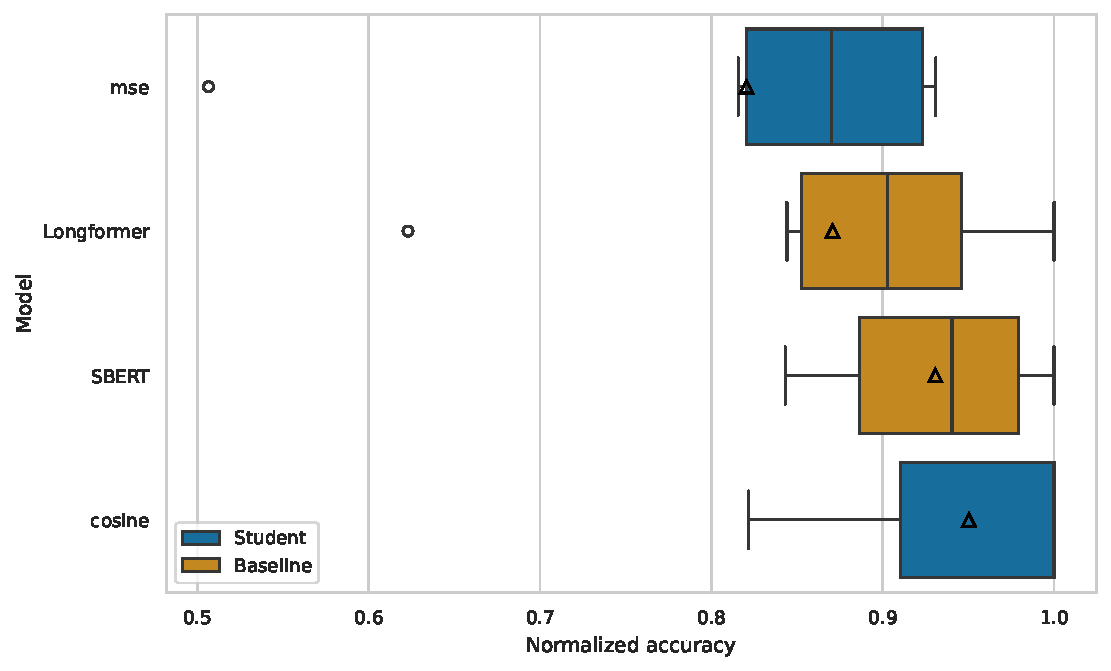
\includegraphics[width=\textwidth]{img/structural_simple_losses.pdf}

  \caption{Performance of student models trained with just the structural
  teacher.}

  \label{fig:structural_basic}
\end{figure}

\subsection{Composite structural losses}\label{section:composite_losses}

Besides the cosine and the MSE, we also explore losses that combine a positive
and a negative component, such as max-marginals or contrastive loss. We call
such losses \emph{composite} as opposed to the \emph{simple} losses, such as
MSE or cosine distance. In composite losses, the positive component compares
the student's and the corresponding teacher's embedding and rewards the model
if they are similar. The negative component compares the student's embedding of
an input and the teacher's embeddings of different inputs and punishes the
model if they are similar. For brevity, we call the teacher's embedding that
correspond to the same input \emph{positive}, while the ones that correspond to
a different inputs \emph{negatives}.

Our initial motivation behind the composite losses was that the negatives could
give the model a more precise indication where it should move its embeddings in
the vector space and therefore it could converge faster to the structural
teacher's embeddings. However, as we discuss in
Section~\ref{section:composite_analysis}, this is not what actually happens.
Nevertheless, some of the models performed so well we do not want to overlook
these losses as they might prove to be beneficial for a future research.

We explored two types of composite losses: max-marginals and contrastive. To
formulate these losses we label the student's embedding as $y$, the
corresponding teacher's embedding as $y_{\text{pos}}$, the set of negatives as
$Y_{\text{neg}}$, the given similarity measure as $\operatorname{sim}$, and a
weighting parameter as $\gamma$. We define the max-marginals loss in
Equation~\ref{eq:max_marginals} and the contrastive loss in
Equation~\ref{eq:contrastive}.


\begin{equation}
  \Loss_{\text{max-marginals}}(y, y_\text{pos}, Y_\text{neg}) =
    \operatorname{sim}(y, y_\text{pos}) -
    \gamma \frac{1}{|Y_\text{neg}|} \sum_{y_\text{neg} \in Y_\text{neg}}
      \operatorname{sim}(y, y_\text{neg})
  \label{eq:max_marginals}
\end{equation}

\begin{equation}
  \Loss_{\text{contrastive}}(y, y_\text{pos}, Y_\text{neg}) =
    -\log \frac{
      \exp(\cos(y, y_\text{pos}))
    }{
      \exp(
        \cos(y, y_\text{pos}) +
        \sum_{y_\text{neg} \in Y_\text{neg}} \cos(y, y_\text{neg})
      )
    }
  \label{eq:contrastive}
\end{equation}

For max-marginals loss, we train with both MSE and cosine distance as
$\operatorname{sim}$ and simultaneously try several weightings $\gamma$. We
compare models trained with the composite losses with those trained with the
simple losses in Figure~\ref{fig:structural_composite_vs_simple}. Composite
losses using MSE, seem to benefit from the negative loss component as 3 out of
4 outperformed the simple MSE loss. However, for only one version, the benefit
  is large enough to outperform the two baselines. With cosine, it seems that
  the negative loss component hurts the performance since only one version
  outperformed the simple cosine loss and it did so by only $10^{-4}$. To
  explain the differences between behaviours of MSE and cosine composite losses
  we carry out an analysis in the subsequent section.

\begin{figure}

  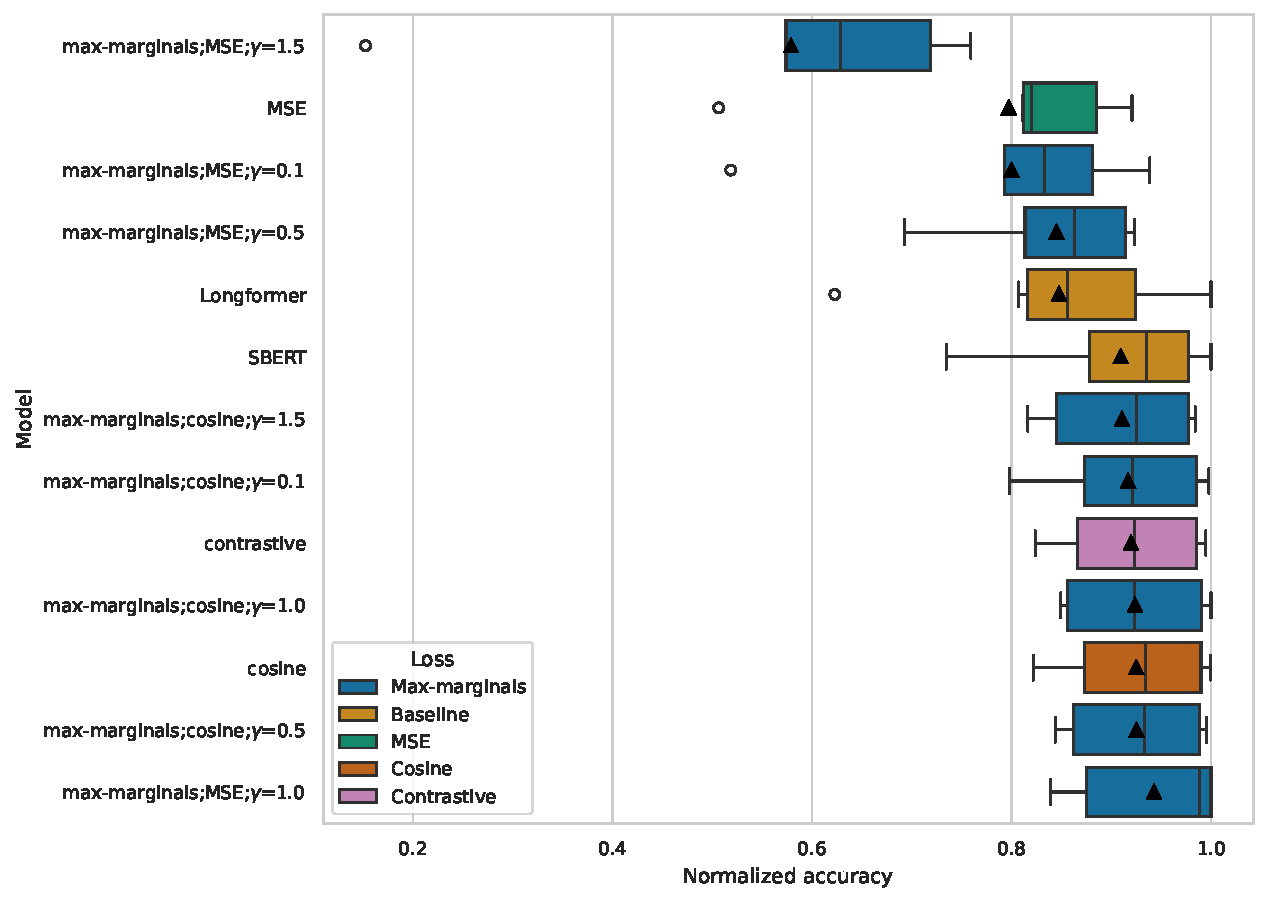
\includegraphics[width=\textwidth]{./img/structural_both_losses.pdf}

  \caption{Performance of student models trained with composite and simple
  structural losses.}

  \label{fig:structural_composite_vs_simple}
\end{figure}

\subsubsection{Analysis of composite losses}\label{section:composite_analysis}

The results of composite losses presented in
Figure~\ref{fig:structural_composite_vs_simple} suggest, that the composite
losses using MSE benefit from the negative loss component, whereas the ones
using cosine do not. Furthermore, for most MSE max-marginals losses the benefit
of negative loss component is only marginal. To explain these results we
compare the distances to positives and negatives for several chosen models in
Figure~\ref{fig:composite_distances}. Composite losses using MSE widen the gap
between positives and negatives at the expense of increasing the distance to
positives. And so, the benefit of the negative component is not that it gives a
more precise training signal and causes a faster convergence to the structural
teacher's embeddings. Conversely, the benefit comes from a clearer separation
between embeddings of different documents, even if the generated embeddings do
not correspond to the teacher's embeddings that well. The situation is
different for cosine, since its range is limited from the top and therefore the
only option how to increase the gap between the positives and the negatives is
to decrease the distances to the positive. Additionally, all of the negatives
are almost perpendicular to the generated embedding and therefore direct the
generated embedding in only one dimension out of the 768. Consequently, the
benefit of the negative component in cosine composite losses is very small.

\begin{figure}
  \centering
  \begin{subfigure}{\textwidth}
    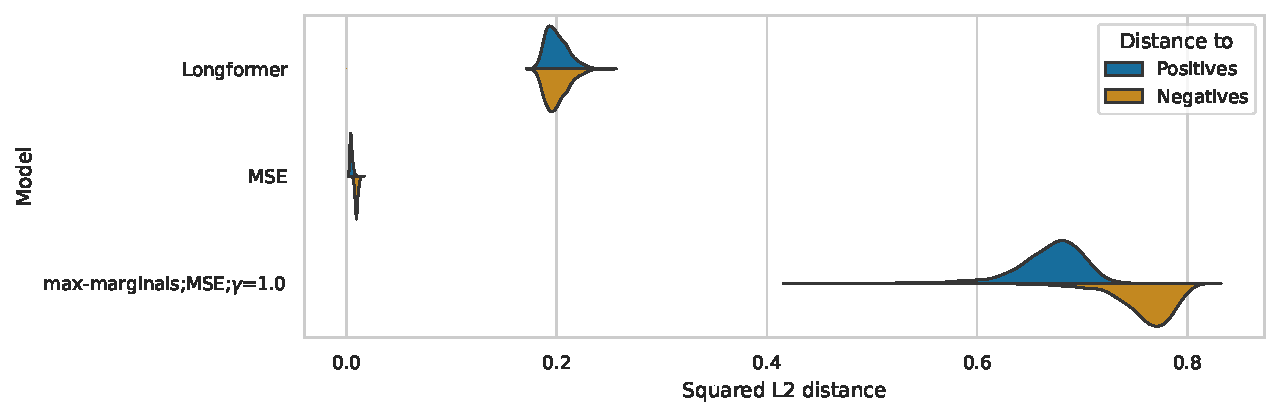
\includegraphics[width=\textwidth]{img/composite_mse_distances.pdf}
    \caption{With MSE}

    \label{fig:composite_mse_distances}

  \end{subfigure}
  \begin{subfigure}{\textwidth}

    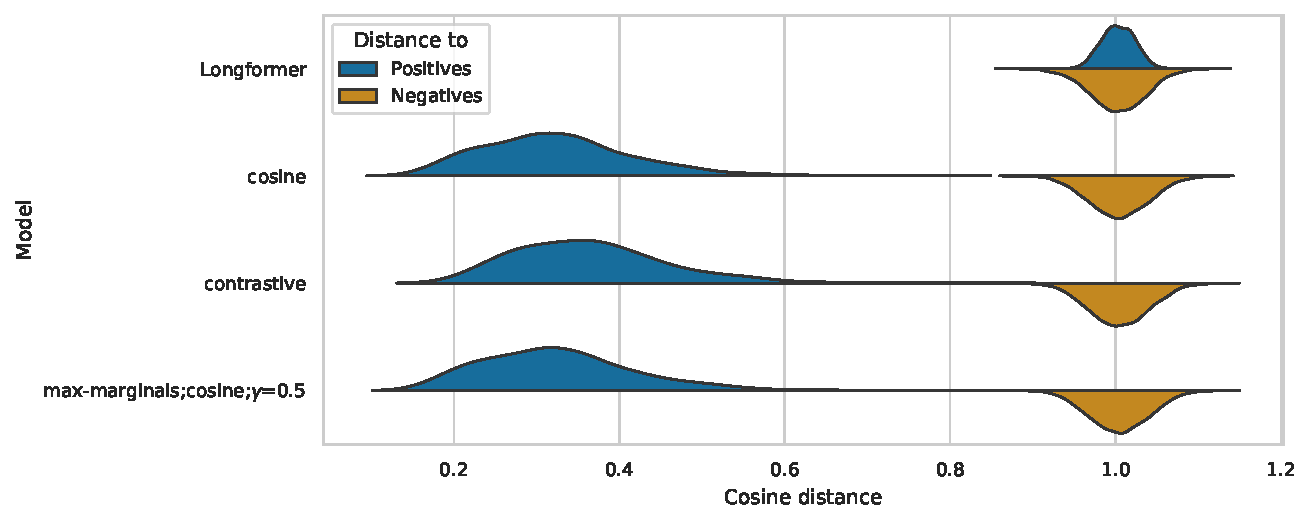
\includegraphics[width=\textwidth]{img/composite_cos_distances.pdf}
    \caption{With cosine}

    \label{fig:composite_cos_distances}
  \end{subfigure}

  \caption{Distribution to distances between the model's and the structural
  teacher's embeddings. A distance to teacher's embedding of the same document
  is labelled as \emph{positive}, whereas distances to teacher's embedding of
  another document is labelled as \emph{negative}. The distances were generated
  from the first 1000 documents of \Dataset{val-500k}'s validation split.}

  \label{fig:composite_distances}

\end{figure}

In summary, contrary to our initial hypothesis, the negative loss component
does not ensure faster convergence of the student's embeddings to those of the
structural teacher. In fact, the negative component causes the student's
embedding to move away from the structural teacher's embedding and hence, goes
against the goal of our training. Nonetheless, as we did not want to throw away
a well-performing model and were interested in how the composite loss would
cooperate with a contextual loss, we continue experimenting the best performing
composite loss in the following sections. Nonetheless, pure cosine loss remains
the preferred structural loss, since it is consistent with the goal of our
training. For brevity we label the student model trained with just the
max-marginals MSE structural loss, with $\gamma=1.0$ as
\Model{only-structural;mm-MSE}.

\section{Structural and contextual loss}\label{section:structural_and_contextual}

In this section, we explore cotextual losses that well complement the best
performing structural and composite structural loss we selected in the previous
section. Since there are quite a few hyperparameters to explore, we split this
section into parts. Each part focuses on a different aspect of the contextual
loss or of the weighting of the contextual and structural loss and selects few
best-performing variants to be explored in the subsequent section. First, in
order to start experimenting with the contextual loss, we need to train the
contextual teacher. We do so in Section~\ref{section:pv_training}, where we
train several Paragraph Vectors and pick the most promising ones. Then we
experiment with the contextual loss's configuration for all selected Paragraph
Vectors in Section~\ref{section:contextual_loss}. We show the performance
attainable only with contextual loss to illustrate how important is the
structural teacher to the student's performance. But more importantly we test
the contextual losses with cosine as well as with max-marginals MSE structural
losses and for each structural loss we pick the best performing combination of
contextual loss configuration and the contextual teacher. Finally, we explore
the weighting of the contextual and structural loss for each of the two
combinations in Section~\ref{section:weighting_experiments}.

\subsection{Optimizing Paragraph Vector's training}\label{section:pv_training}

We choose Paragraph Vector \citep{le2014distributed} as our contextual teacher,
as we elaborate on in Section~\ref{section:paragraph_vector}. Since there is no
concept of a pre-trained PV, as in the case of transformers, we train PV from
scratch. We use PV's implementation from Gensim
library\footnote{\label{fn:link_to_gensim}\url{https://radimrehurek.com/gensim}}
and explore some of the hyperparameters that govern the training of PV. We
focus on four hyperparameters that we consider important, and adopt the
recommendation of either the library or related literature. Both the adopted
and the grid-searched hyperparameters are enumerated in
Table~\ref{table:pv_hyperparams}. To explain the meaning of all hyperparameters
we provide the following summary:


\begin{itemize}

  \item \texttt{dm} --  PV architecture; true for Distributed Memory (DM),
    false for Distributed Bag of Words (DBOW)

  \item \texttt{vector\_size} -- dimensionality of the generated embedding

  \item \texttt{min\_count} -- words with document frequency below this limit
    will be ignored

  \item \texttt{text\_pre\_process} -- applied word processing done before the
    model's training; for stemming we used PorterStemmer implemented by
    \texttt{nltk}
    library\footnote{\url{https://www.nltk.org/api/nltk.stem.porter.html}}

  \item \texttt{negative} -- number of noise words used for negative sampling
    during training

  \item \texttt{window} -- the maximum distance between known and predicated
    word

  \item \texttt{sample} -- percentile threshold configuring which words will be
    downsampled; 0 for no downsampling


  \item \texttt{dbow\_words} -- whether to train word embeddings using
    Word2Vec's \citep{mikolov2013efficient} Skip-gram architecture together
    with document embeddings; only applicable to DBOW, as DM learns word
    embeddings by default

  \item \texttt{epochs} -- number of iterations done over the corpus during
    training

\end{itemize}


As recommended by the authors of PV \citep{le2014distributed}, we experiment
with both architectures. For each architecture we try different settings of
\texttt{vector\_size}, \texttt{min\_count} and \texttt{text\_pre\_process},
which all control the regularization of the model. Settings such as higher
dimensional embedding, small minimum count and no text pre-processing,
regularize the model the least. They give the model the most information on its
inputs, while also providing it with large embedding through which the model
can express precisely. On the other hand, using lower dimensional embedding,
large minimum count and stemming the document's words, forces the model to be
more general and less precise. The model has less detailed information on its
input and must squeeze all of it to a small vector. We did not see any value in
trying dimensions of embeddings higher than 1024 as in later experiments we
need to distill the contextual embedding to a 768-dimensional embedding of our
student model. Intuitively, the larger the contextual embedding is going to be,
the smaller the fraction of information the student model is going to be able
to digest. Also there is no value in considering \texttt{min\_count} to be
lower than 2, since we would only add words that are unique to a single
document. Embeddings of such words would be poorly trained and would not add
meaningful information to the document's embedding. Last hyperparameter that is
worth mentioning is \texttt{dbow\_words}. DBOW on its own does not train word
embeddings, which are randomly generated. Setting \texttt{dbow\_words} to true
causes DBOW to also train word embeddings using Word2Vec's Skip-gram model
\citep{mikolov2013efficient} in each epoch. \cite{lau2016empirical} showed that
random word embeddings significantly hurt the model. Consequently, when
training DBOW we also train word embeddings, despite the longer training, which
it inevitably causes.

\begin{table}
  \footnotesize
  \centering
  \begin{tabular}{lrc}
    \toprule
    Hyperparameter & Value(s) & Recommended by \\
    \midrule
    \texttt{dm} & true, false & - \\
    \texttt{vector\_size} & 100, 768, 1024 & - \\
    \texttt{min\_count} & 2, 10\% of train corpus & - \\
    \texttt{text\_pre\_process} & stem, lowercase, none & - \\
    \texttt{window} & 5 & default \\
    \texttt{negative} & 5 & default, \cite{lau2016empirical} \\
    \texttt{sample} & 0 & default \\
    \texttt{dbow\_words} & true & \cite{lau2016empirical} \\
    \texttt{epochs} & 10 & default, \cite{dai2015document} \\
    \bottomrule
  \end{tabular}

  \caption{Used hyperparameters for training Paragraph Vector. We grid-searched
  four hyperparameters: PV architecture, vector size, minimum word count and
  pre-processing of words. The rest of the hyperparameters we adopted either the
  default values or recommended by the mentioned literature.}

  \label{table:pv_hyperparams}

\end{table}

We train all variants on whole \Dataset{val-500k} corpus. We follow the
recommendations of \cite{le2014distributed} and test also the combination of
both architectures, where the resulting embedding is a concatenation of
embeddings of the combined models. However, we only select the best 3 models
from each architecture and evaluate all 9 combinations. We call these models
\emph{compound} Paragraph Vectors. In total there are 45 models, whose
performance on validation tasks we report in Figure~\ref{fig:pv_val_scores}.
Among the single models, large embedding dimensions and low minimum count were
favored. Additionally, on average, stemming or lowercasing lead to higher score
than not pre-processing the words at all. DBOWs vary more in performance,
occupying the best and the worst positions, whereas DMs are a bit more
consistent. We achieve a slight improvement by concatenating a DM and a DBOW
model, but considering the resulting model has effectively double the embedding
size, the improvement is not surprising. Interestingly, all compound models
perform very similarly, suggesting that slight imperfections of one model can
be compensated by another model of a different architecture.

\begin{figure}

    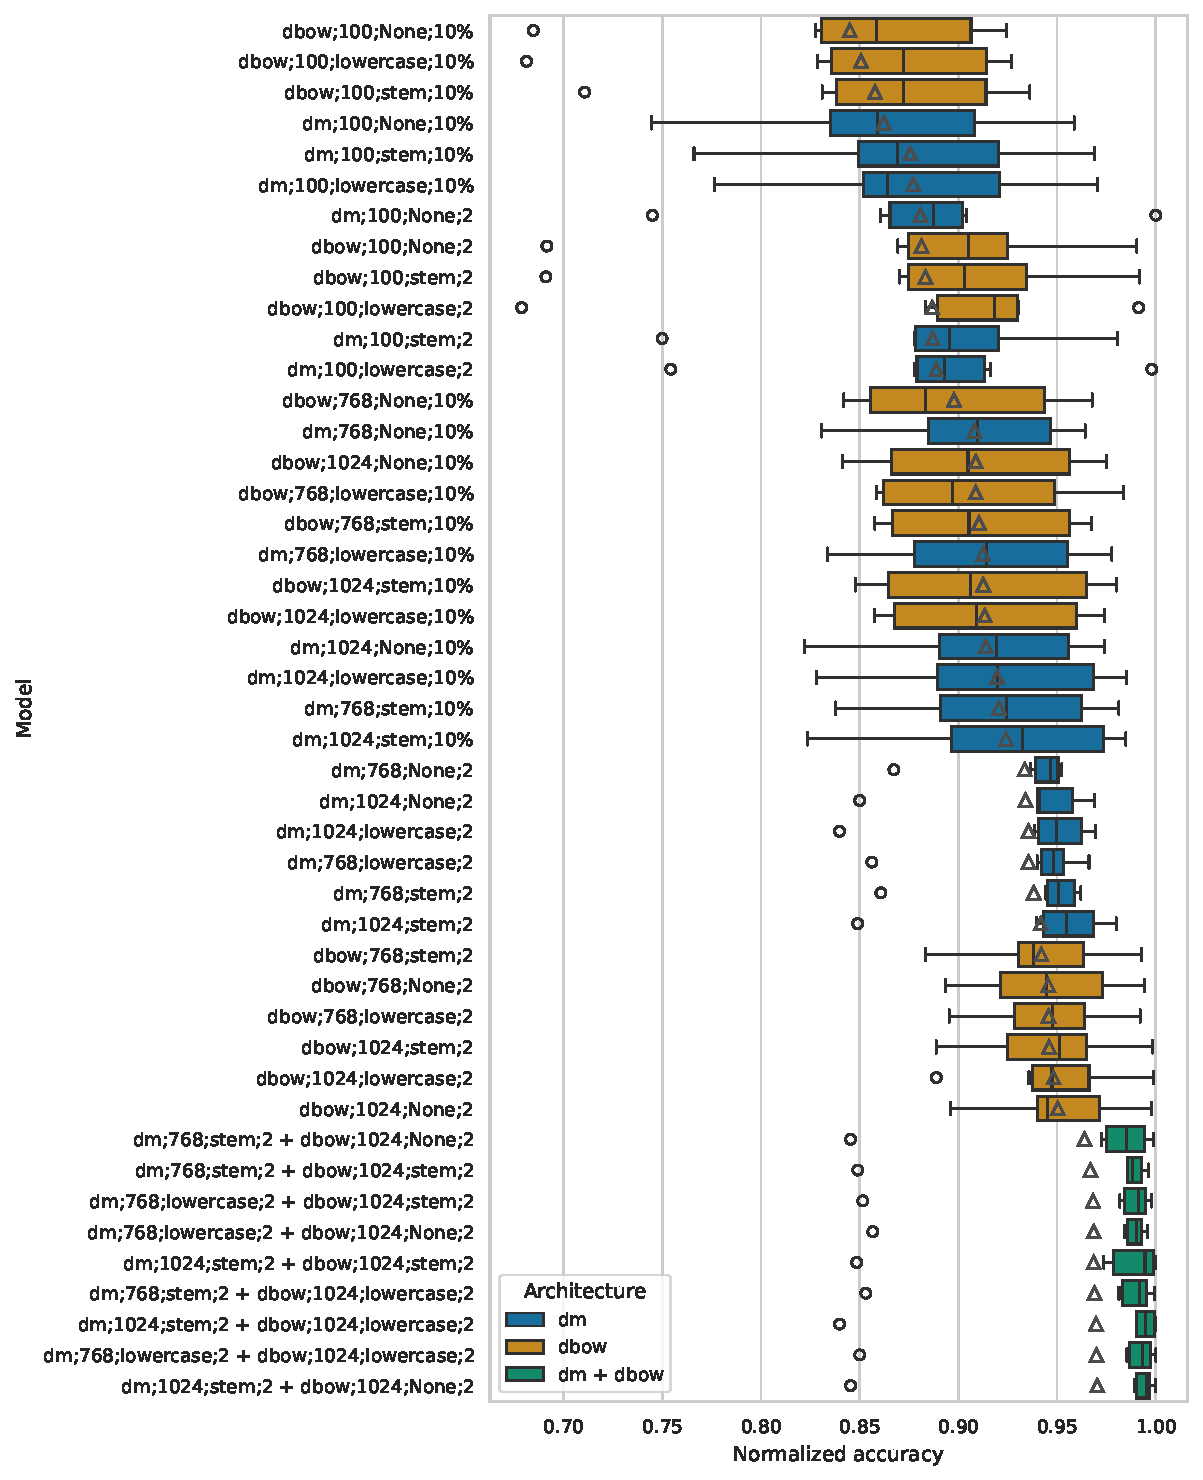
\includegraphics[width=\textwidth]{./img/pv_val_scores.pdf}

    \caption{Performance of all Paragraph Vector variants on validation tasks.
    A model is identified by architecture, embedding dimension, text
    pre-processing and minimum count, in this order. Models composed of two
    sub-models are identified as a concatenation of such identifiers separated
    by $+$.}

    \label{fig:pv_val_scores}

\end{figure}

In our preliminary experiments we saw that the dimension of the contextual
teacher's embedding plays a significant role in the teacher-student training.
And so we select three Paragraph Vectors with varying vector sizes. We pick the
best model with small vector size (\Model{DM;100;lowercase;2}), the best
single model (\Model{DBOW;1024;None;2}) and the best model composed of both
architectures (\Model{DM;1024;stem;2+DBOW;1024;None;2}). For brevity we label
these models as \Model{DM;100d}, \Model{DBOW;1024d} and \Model{PV;2048d}.

\subsection{Contextual loss}\label{section:contextual_loss}

Contextual loss $\Loss_C$ compares the student's and the contextual teacher's
embeddings and encourages distillation of the quality of the teacher's
embedding into the student's embedding. As we discuss in
Section~\ref{section:abstract_loss}, we choose $\Loss_C$ to be less strict and
give the student model more freedom in how it encodes information into the
document embedding. Consequently we do not consider losses such as MSE, or
cosine, since they enforce either an exact vector or a direction in the
embedding space. Instead we use a variant of \emph{Canonical Correlation
Analysis} \citep{hotelling1992relations} (\emph{CCA}). In its base form CCA
computes a correlation of two linearly projected sets of vectors, where the
projections are optimized so that the correlation is maximized. We define CCA
in Equation~\ref{def:cca_more_dim}.

\begin{defn}[Canonical Correlation Analysis]\label{def:cca_more_dim}

  For two matrices $X_1 \in \mathbb{R}^{n_1 \times m_1}$ and $X_2 \in
  \mathbb{R}^{n_2 \times m_1}$, Canonical Correlation Analysis for $k$
  dimensions finds $P \in \mathbb{R}^{m_1 \times k}$ and $Q \in \mathbb{R}^{m_2
  \times k}$ that maximize

  \begin{equation}
    \begin{split}
      &\CCA(X_1, X_2) = \sum_{i = 1}^k \corr(X_1P_{*i}, X_2Q_{*i}) \\
      \text{s.t.}\quad &P^TX_1^TX_1P = I_k = Q^TX_2^TX_2Q \\
    \end{split}
  \end{equation}


\end{defn}

CCA gives the student the freedom to change its embeddings as long as their
linear projections correlate more with the linear projections of the contextual
teacher's embeddings. However, linear projection may still leave too little
leeway for the student model to simultaneously mimic the structural teacher,
while increasing the correlation with the projected contextual teacher's
embeddings. Ideally we would like to adjust the strength of the projections and
thus enforce more or less exact correlation between the student's and the
teacher's embeddings. Such adjustment is possible with \emph{Deep CCA}
(\emph{DCCA}) \citep{andrew2013deep}. DCCA projects the input vectors with two
neural networks, and then feeds the projections to the vanilla CCA. The two
networks are simultaneously trained together with the embedding model based on
the computed CCA, which is used as a loss. The advantage of DCCA is that we can
adjust the strength of the projections and thereby regulate pressure the
contextual loss inflicts on the student model. The larger the neural network
is, the more it is going to be able to transform the embeddings and the less is
the student model going to need adjust its embedding.

As we can see in Equation~\ref{def:cca_more_dim}, CCA is computed from the
entire dataset of input vectors. And so, DCCA is trained using a full-batch
optimization \citep{andrew2013deep} or a mini-batch optimization with large
batch sizes \citep{wang2015unsupervised}. However, both methods need large
amount of GPU memory and therefore are applicable only to small models. For
this reason we avoid CCA and use SoftCCA \citep{chang2018scalable} instead,
which reformulates CCA, such that it is usable even in case of mini-batch
optimization with small batches. To explain how SoftCCA is related to CCA we
reformulate the solution to CCA using a Forbenious matrix norm in
Equations~\ref{def:cca_with_forbenious_first}-\ref{def:cca_with_forbenious_last}.

\begin{align}
  P^\ast, Q^\ast &= \underset{P, Q}{\argmin} ||X_1P - X_2Q||^2_F \label{def:cca_with_forbenious_first} \\
  &= \underset{P, Q}{\argmin} \trace\left((X_1P - X_2Q)^T(X_1P - X_2Q)\right) \\
  &= \underset{P, Q}{\argmin} {-2} \trace(P^TX_1^TX_2Q) \\
  &= \underset{P, Q}{\argmax} \trace(P^TX_1^TX_2Q) \\
  &= \underset{P, Q}{\argmax} \sum_{i = 1}^k \corr(X_1P_{*i}, X_2Q_{*i}) \label{def:cca_with_forbenious_last}
\end{align}

Thus, by minimizing CCA we effectively minimize the difference between two
projections with uncorrelated features. SoftCCA mimics these two effects with
two separate losses:

\begin{itemize}

  \item L2 loss which minimizes of the difference between projections:

    \begin{equation}
      \Loss_{\text{L2}}(X_1, X_2) = ||X_1 - X_2||^2_F = \MSE(X_1, X_2)
    \end{equation}

  \item \emph{Soft Decorrelation Loss} (\emph{SDL}) which forces a projection
    to have decorrelated features:

    \begin{equation}
      \Loss_{\text{SDL}}(X^t) = \sum_{i \ne j} \left|
          \frac{(\Phi^t_X)_{ij}}{\hat{\beta}^t}
          \right|
    \end{equation}
    where
    \begin{align}
      \Phi^t_X &= \beta \Phi^{t-1}_X + \Sigma_{X^t} \\
      \Phi^0_X &= \bm{0}_d \\
      \hat{\beta}^t &= \beta \hat{\beta}^{t-1} + 1 \\
      \hat{\beta}^0 &= 0
    \end{align}

\end{itemize}

Where

\begin{itemize}

  \item $X, X_1, X_2 \in \mathbb{R}^{b \times d}$ are mini-batches of
    $d$-dimensional vectors

  \item $\Sigma_{X}$ is a covariance matrix of a mini-batch of vectors $X$

  \item $\bm{0}_d$ is a $d \times d$ zero matrix

  \item $\beta$ is a hyperparameter

  \item $\Phi_X^t, X^t, \hat{\beta}^t$ is $\Phi_X, X, \hat{\beta}$ at iteration
    $t$

\end{itemize}

The L2 loss forces the projected vectors to be equal, while the Soft
Decorrelation Loss forces them to have uncorrelated features. Notice that to
have a better estimate of the projected vector's covariance matrix, SDL keeps a
running mean. Similarly to Batch Normalization \citep{ioffe2015batch}, SDL
updates the running mean during training, but avoids any updates during
inference. With the above losses, and the weighting hyperparameter
$\delta$, we define SoftCCA in Equation~\ref{eq:soft_cca}.

\begin{equation}\label{eq:soft_cca}
  \Loss_{\text{SoftCCA}}(X_1, X_2) = \Loss_{\text{L2}}(X_1, X_2) +
      \delta ( \Loss_{\text{SDL}}(X_1) + \Loss_{\text{SDL}}(X_2) )
\end{equation}

We use SoftCCA loss as a replacement for CCA in DCCA. To be explicit, we
project the student's and the contextual teacher's embedding with two separate
feed-forward neural networks and then apply SoftCCA loss, which provides
training signal not only for the embedding model, but also for the neural
networks projecting the embeddings. For brevity we call the neural networks
that project the student's and the contextual teacher's embedding
\emph{student} and \emph{contextual projections}, respectively. And so, we can
finally express $\Loss_C$ from Equation~\ref{eq:abstract_loss} more concretely.
For a student projection $f_\Student$ and a contextual projection $f_C$, we
formulate our contextual loss in Equation~\ref{eq:contextual_loss}. We also
illustrate the architecture of contextual loss graphically in
Figure~\ref{fig:contextual_loss}.

\begin{equation}\label{eq:contextual_loss}
  \Loss_C(y_\Student, y_{\Teacher_C}) = \Loss_{\text{SoftCCA}}(
    f_\Student(y_\Student),
    f_C(y_{\Teacher_C})
  )
\end{equation}

\begin{figure}

  \centering
  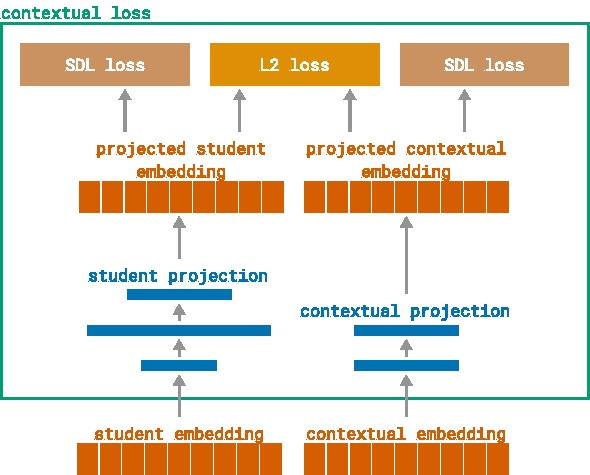
\includegraphics[width=0.7\textwidth]{img/contextual_loss.pdf}

  \caption{Architecture of contextual loss.}

  \label{fig:contextual_loss}

\end{figure}

In our preliminary experiments, we found that the value of $\delta$ from
Equation~\ref{eq:soft_cca} has little effect on the final student's
performance. So, we set it so that the ranges of $\Loss_{\text{L2}}$ and
$\Loss_{\text{SDL}}$ are roughly equal and leave it as so. On the other hand,
choosing a correct value of $\beta$ showed to be critical. Based on how the CCA
of the projected embeddings of the validation split progressed throughout the
training, we found the optimal value to be 0.95, which puts relatively large
emphasis on the accumulated mean compared to lower values of $\beta$.

In the rest of this section, we experiment with the strength of the
projections. In the following section we build the basic intuition behind
training with the two projections and SoftCCA, while finding the ideal
contextual projection without any structural loss. In the subsequent sections
we study how different structural losses influence the projections. First we
experiment with cosine and then with max-marginals MSE loss. In all cases we
test the projections for each of the three contextual teachers:
\Model{DM;100d}, \Model{DBOW;1024d} and \Model{PV;2048d}. At the end, we select
the best contextual loss with the best contextual teacher for both cosine and
max-marginals MSE structural loss, with which we experiment further later in
this chapter.

\subsubsection{Contextual projection with contextual loss
only}\label{section:projections_only_contextual}

With only the contextual loss, the student's only goal is to mimic the
contextual teacher. This presents a very basic setting, in which we can study
the behaviour of the projections and of the contextual loss as a whole without
any influence from the structural loss.

As we learned in our preliminary experiments over-parameterization of the
projections hurts the performance of the model. Even though large projections
result in smaller SoftCCA loss, they tend to harm the CCA of the student's and
contextual teacher's embeddings. Strong projections compensate for the
student's flaws, which lessens the pressure on the student model as it does not
need to adjust its embedding that much. As a consequence, the student model
learns very little compared to the projections. Similarly, strong contextual
projection take away pressure from the student projection and vice-versa. In
this regard, it is important to keep the contextual projection small, and
therefore put more pressure on the student's side where the gradients can
propagate to the embedding model itself.

As we mentioned before, we feed the projected outputs to SoftCCA loss
$\Loss_{\text{SoftCCA}}$. As SoftCCA requires both inputs to be of the same
dimension, both projections must end with an equally sized layer. We always use
the dimension of the larger embedding as the final projection dimension. We do
so, to preserve all the embedding's information through the projection and
force the student model to distill all of the dimensions of the contextual
embedding and not just their subset. Also there is no point in projecting the
embeddings to even more dimensions than the embeddings have originally. Due to
the Pigeonhole principle, some features of the final projections would have to
depend on the same embedding's features and therefore would correlate with each
other. This would create unnecessary conflict with the SDL loss, which forces
the projections to output uncorrelated features. This phenomenon would also
occur for projections that have a shape of an hourglass, where there is a one
bottle-neck layer with significantly less dimensions than the layers after or
before it. And indeed, during preliminary testing, we saw these projections to
always perform poorly.

We build the projections as a sequence of blocks, where each block is composed
of a fully connected layer and a optional Rectified Linear Unit (\emph{ReLU}).
In preliminary experiments, we also tried adding Dropout, Batch or Layer
Normalization layers at different places in a block, but they have either
negligible or negative effect on the performance of the final model. We label
each block with the dimension of the fully connected layer and with the
activation's name in brackets if it is used. The whole projection is then
identified by block's labels delimited by an ``x''. So, \Proj{768(ReLU)x1024}
are two feed forward layers with 768 and 1024 features connected via ReLU. To
label projections without any layers we use a dash. We present all the
projections' variations we tested in Table~\ref{table:contextual_projections}.
Considering the conditions we describe in previous paragraph, we choose a
strong and a weak projection for both student and contextual side. We are
careful not to over-parametrize either projection, and lean toward stronger
student projection.

\begin{table}
  \centering
  \footnotesize

  \begin{tabular}{lrrr}
    \toprule
      & \multicolumn{3}{c}{Contextual teacher's embedding dimension} \\
      \cline{2-4} \\
      Projection & 100 & 1024 & 2048 \\
    \midrule
      \multirow[t]{2}*{Student} & \Proj{768(ReLU)x1024(ReLU)x768} & \Proj{768(ReLU)x1024} & \Proj{1024(ReLU)x2048} \\
      & \Proj{768} & \Proj{1024} & \Proj{2048} \\
      \multirow[t]{3}*{Contextual} & \Proj{100(ReLU)x768} & \Proj{768x1024} & \Proj{1024x2048} \\
      & \Proj{768} & \Proj{1024} & \Proj{2048} \\
      & & - & - \\
    \bottomrule
  \end{tabular}

  \caption{All tested variants of projections with only contextual loss. We do
  a grid search of the given variants for each contextual teacher. This results
  in 16 combinations overall.}

  \label{table:contextual_projections}
\end{table}

We train the student models on the first 15k documents of \Dataset{val-500k}
and compare the models' performance to all the relevant teachers, Longformer
and \Model{only-structural;cosine} in Figure~\ref{fig:projections_contextual}.
We identify a student model with the contextual teacher's dimension, the
student projection prefixed by \Model{S:} and the contextual projection
prefixed by \Model{C:}.

The results correspond to those we witnessed in our preliminary experiments and
showcase some of the mentioned projections' behaviours. The better half of the
student models differs from the rest by having a minimal contextual projection.
Moreover, for a given contextual teacher and a projection, the student model
with larger student projection outperforms the student with a smaller one in
all cases but one.

Half of the tested projections improve the score of Longformer. This suggests
that we are able to distill useful information from the contextual teacher to
the student and also highlights the importance of a good projection. However,
as our contextual loss does not enforce exact similarity of the student's and
the contextual teacher's embedding, most of the students do not outperform
their respective contextual teachers. Interestingly, students trained with
\Model{DM;100d} surpass students trained with better performing
\Model{DBOW;1024d}. We can observe the same performance differences for
\Model{DBOW;1024d} and \Model{PV;2048d}, even if we compare projections that
scale with the contextual embedding, such as \Proj{1024d;S:1024;C:-} and
\Proj{2048d;S:2048;C:-} or \Proj{1024d;S:1024;C:1024} and
\Proj{2048d;S:2048;C:2048}. Consequently, it seems that it is easier to distill
information from an embedding with less features than from a larger one. And
so, even though PV with 2048 dimensions beats SBERT, the students trained with
it fail to capitalize on this advantage and perform worse than the model
trained with SBERT. Therefore, we conclude that according to our results the
structural teacher is more important to the student's performance than the
contextual teacher and justifies why we search for the ideal contextual loss to
the best performing structural loss rather than the other way around.

\begin{figure}

  \centering

  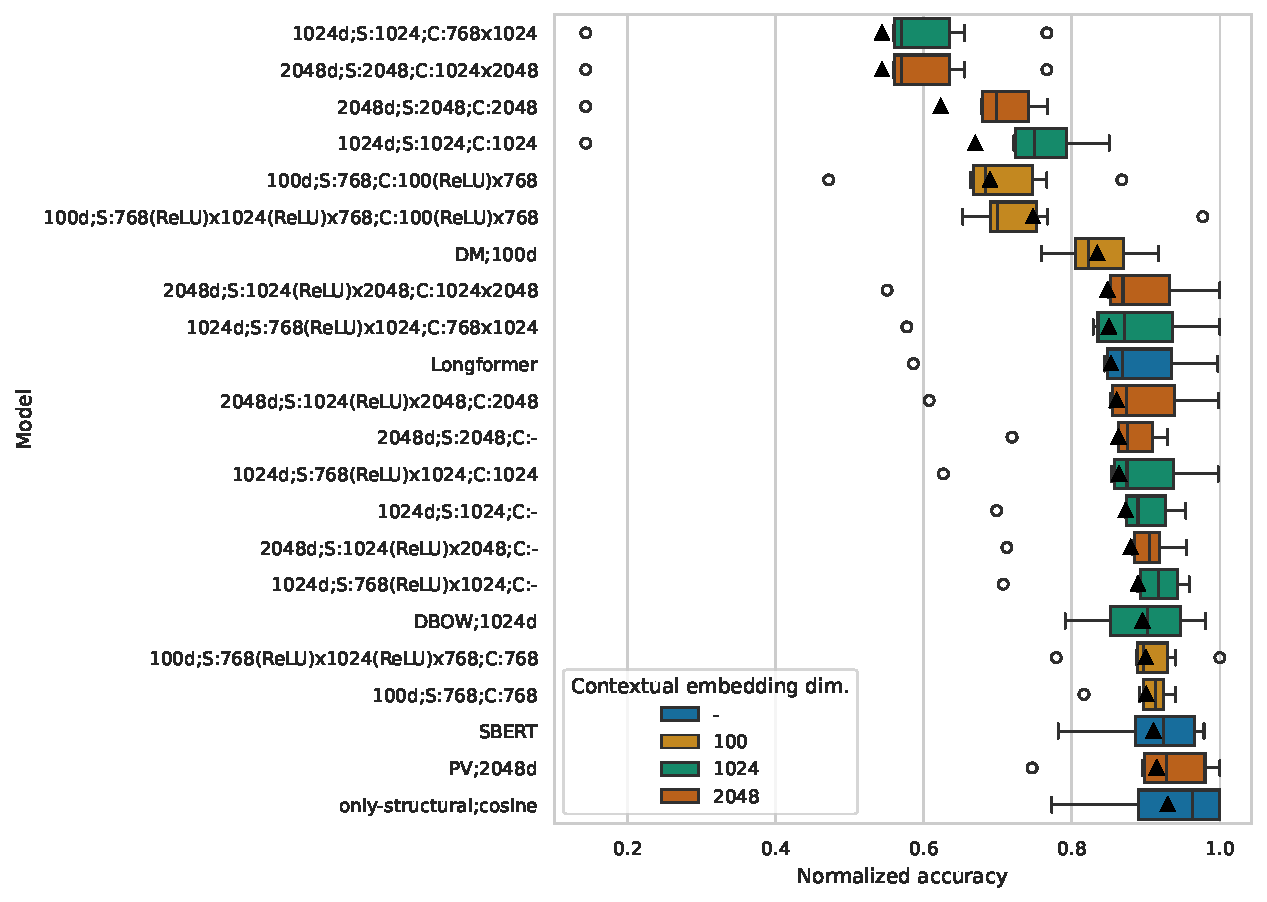
\includegraphics[width=\textwidth]{img/projections_contextual.pdf}

  \caption{Performances of student models trained with different projections
  and without any structural loss. We compare the students to all the relevant
  teachers, Longformer and \Model{only-structural;cosine}.}

  \label{fig:projections_contextual}

\end{figure}

\subsubsection{Contextual projection with cosine structural
loss}\label{section:projections_cos}

We now search for the best performing projections while simultaneously using
cosine structural loss. Compared to the previous section, the training is a bit
more complex as the student is now forced to distill two qualities, each from a
different teacher. So, even though the student and contextual
projections still behave in the same manner, they may cause different outcomes.

We list all the tested projections in
Table~\ref{table:cos_contextual_projections}. We add stronger projections,
while discarding some of the less successful projections from the previous
section. We again train the student models on the first 15k documents of
\Dataset{val-500k} and present the performance of the trained student models in
Figure~\ref{fig:cos_projections_contextual}. Compared to the student models
trained without any structural loss, the same projection variants differ less.
The cosine structural loss boosts the models' performance and lessens the
negative impact of a poor projection. As a consequence, almost all of the
student models surpass all baselines. The best performing projections are much
larger compared to the best projections trained without any structural loss.
This seems logical, as the added structural loss puts more pressure on the
student, and so the contextual loss needs to give the model more freedom in
order to avoid conflict between the losses, which would slow down the training.
With the larger projections we were able to surpass
\Model{only-structural;cosine}. This shows that, with well performing
projections, the student model benefits from both losses being used during
training. Even if the performance gain is not huge, we conclude that the
contextual and structural embeddings complement each other.

\begin{table}
  \centering
  \footnotesize

  \begin{subtable}{\textwidth}
    \centering
    \begin{tabular}{lr}
      \toprule
        & Contextual teacher's embedding dimension \\
        \cline{2-2} \\
        Projection & 100 \\
      \midrule
        Student & \Proj{768(ReLU)x1024(ReLU)x768}  \\
        \multirow[t]{2}*{Contextual} & \Proj{100(ReLU)x768}  \\
        & \Proj{768} \\
      \bottomrule
    \end{tabular}
    \caption{100 dimensional contextual teacher}
  \end{subtable}
  \medskip

  \begin{subtable}{\textwidth}
    \centering
    \begin{tabular}{lrr}
      \toprule
        & \multicolumn{2}{c}{Contextual teacher's embedding dimension} \\
        \cline{2-3} \\
        Projection & 1024 & 2048 \\
      \midrule
        Student &  \Proj{768(ReLU)x1024} & \Proj{1024(ReLU)x2048} \\
        \multirow[t]{2}*{Contextual} &  \Proj{1024} & \Proj{2048} \\
        & - & - \\
      \midrule
        Student & \Proj{768(ReLU)x4096(ReLU)x1024} & \Proj{768(ReLU)x4096(ReLU)x2048} \\
        \multirow[t]{3}*{Contextual} & \Proj{768(ReLU)x1024} & \Proj{2048(ReLU)x2048} \\
        & \Proj{1024} & \Proj{2048} \\
        & - & - \\
      \bottomrule
    \end{tabular}

    \caption{1024 and 2048 dimensional contextual teachers}

  \end{subtable}

  \caption{All tested variants of projections with contextual loss and cosine
  structural loss. For a given contextual teacher, we delimit each group of
  projections by a horizontal line. We grid search all variants within each
  group. This results in 12 combinations of projections.}

  \label{table:cos_contextual_projections}
\end{table}

\begin{figure}

  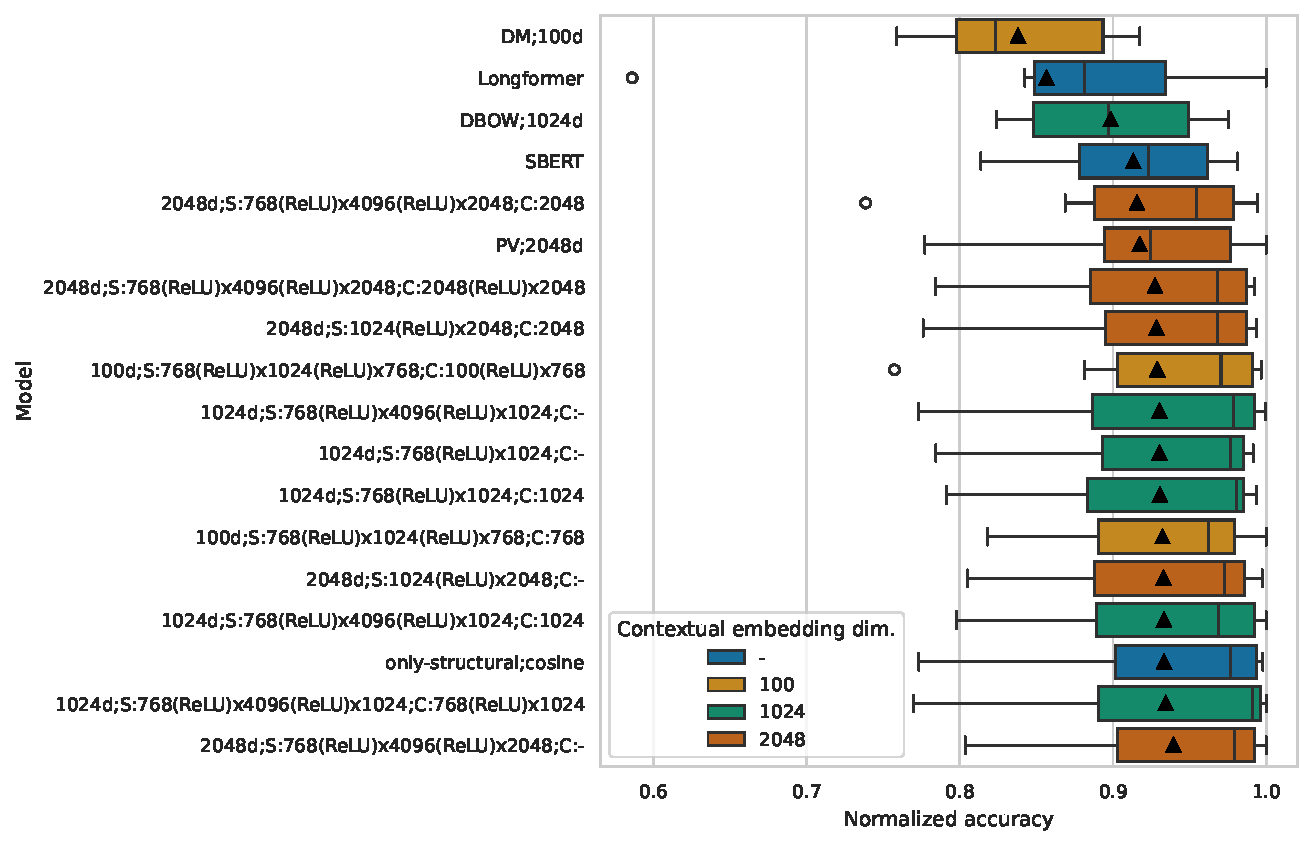
\includegraphics[width=\textwidth]{img/projections_contextual_cos.pdf}

  \caption{Performance of student models trained with contextual and cosine
  structural loss on validation tasks. We compare the student models to all
  relevant teachers, Longformer and \Model{only-structural;cosine}.}

  \label{fig:cos_projections_contextual}

\end{figure}

\subsubsection{Contextual projection with max-marginals MSE structural
loss}\label{section:projections_mm_mse}

We also search for optimal projections when simultaneously training with the
max-marginals MSE loss. Although, as we show in
Section~\ref{section:composite_analysis}, max-marginals MSE structural loss
goes against the goal of our student-teacher training, it surpassed all the
composite and the simple structural losses. We continue experimenting with it
here, to see how does the student react to different configuration of the contextual loss.

We present all the tested projection variants in
Table~\ref{table:mm_mse_contextual_projections}. We included successful
projections from previous section and add stronger contextual projections as
they perform in this context surprisingly well. Same as before, we train all
student models on the first 15k documents from \Dataset{val-500k} and compare
their performance to all relevant teachers, Longformer and
\Model{only-structural;mm-MSE}. We present the model's performances in
Figure~\ref{fig:mm_mse_contextual_projections}. As is the case with the cosine
structural loss, max-marginals MSE loss boosts the students' performances.
Consequently, we see that the student's performances are not as dependent on
the projections as much as in the case of students trained without any
structural loss. Contrary to what we witness in previous experiments, stronger
contextual projections perform overall very well. This shows that max-marginals
with MSE exerts so much pressure on the student's embedding the projections
need to be even stronger than in the case of cosine structural loss. Again we
find the max-marginals MSE structural loss to not quite correspond with our
training technique. As a consequence and despite testing even more projections
than in the case of cosine structural loss, we fail to find projections with
which would the student benefit from both contextual and max-marginals MSE
structural losses used during training.

\begin{table}
  \centering
  \footnotesize

  \begin{subtable}{\textwidth}
    \centering
    \begin{tabular}{lr}
      \toprule
      % TODO: name the same in the chart or rename it here
        & Contextual teacher's embedding dimension \\
        \cline{2-2} \\
        Projection & 100 \\
      \midrule
        \multirow[t]{2}*{Student} & \Proj{768(ReLU)x1024(ReLU)x768}  \\
        & \Proj{768} \\
        \multirow[t]{2}*{Contextual} & \Proj{100(ReLU)x768}  \\
        & \Proj{768} \\
      \bottomrule
    \end{tabular}
    \caption{100 dimensional contextual teacher}
  \end{subtable}
  \medskip

  \begin{subtable}{\textwidth}
    \centering
    \begin{tabular}{lrr}
      \toprule
        & \multicolumn{2}{c}{Contextual teacher's embedding dimension} \\
        \cline{2-3} \\
        Projection & 1024 & 2048 \\
      \midrule
        Student &  \Proj{768(ReLU)x1024} & \Proj{1024(ReLU)x2048} \\
        \multirow[t]{3}*{Contextual} & \Proj{768x1024} & \Proj{1024x2048} \\
        & \Proj{1024} & \Proj{2048} \\
        & - & - \\
      \midrule
        Student & \Proj{768(ReLU)x4096(ReLU)x1024} & \Proj{768(ReLU)x4096(ReLU)x2048} \\
        \multirow[t]{3}*{Contextual} & \Proj{1024(ReLU)x1024} & \Proj{2048(ReLU)x2048} \\
        & \Proj{768(ReLU)x1024} & - \\
      \bottomrule
    \end{tabular}

    \caption{1024 and 2048 dimensional contextual teachers}

  \end{subtable}

  \caption{All variants of projections tested together with
  max-marginals MSE structural loss. For a given contextual teacher, we delimit
  each group of projections by a horizontal line. We grid search all variants
  within a group. This results in 14 combinations in total.}

  \label{table:mm_mse_contextual_projections}
\end{table}

\begin{figure}

  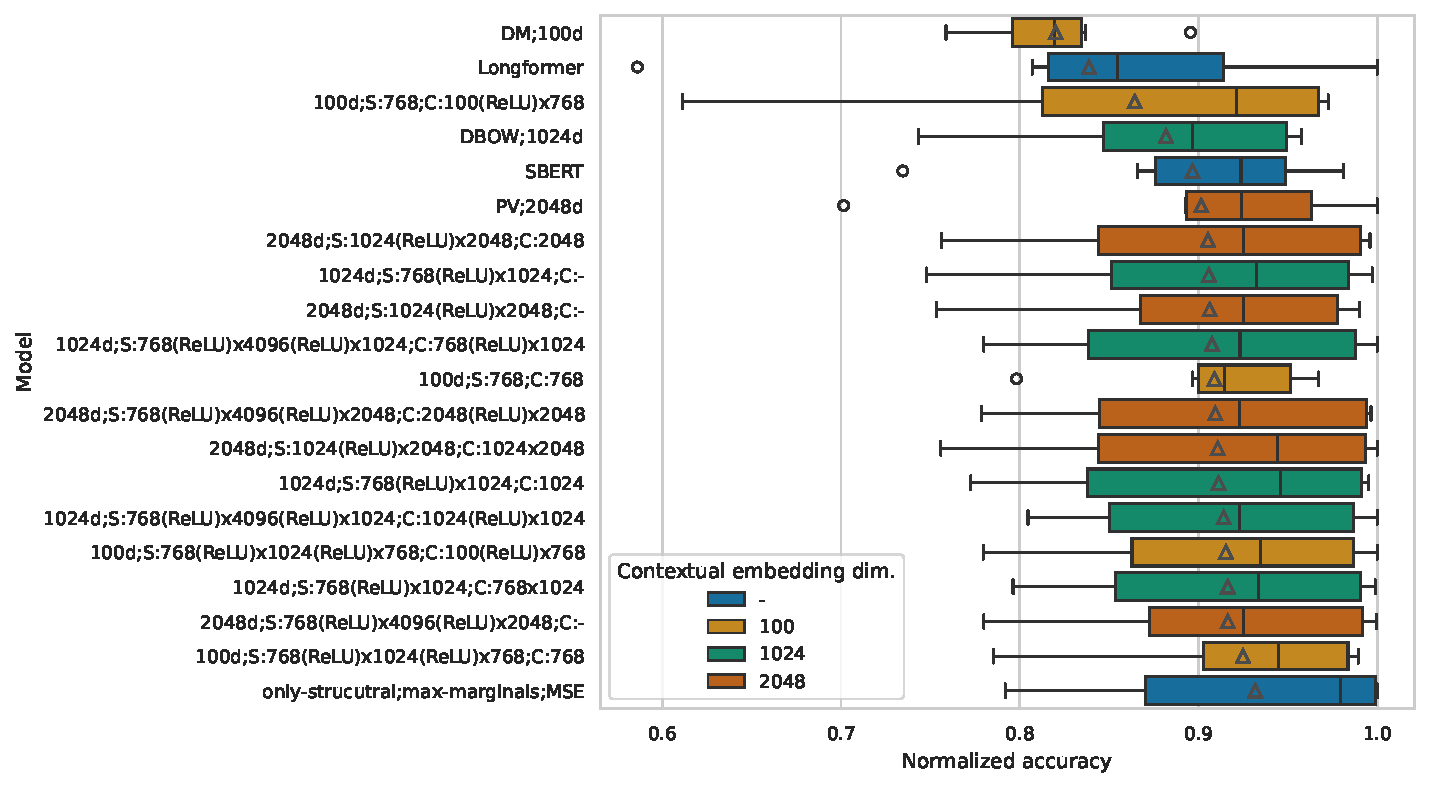
\includegraphics[width=\textwidth]{img/projections_contextual_mm_mse.pdf}

  \caption{Performance of student models trained with contextual and
  max-marginals MSE structural loss on validation tasks. We compare the student
  models to all relevant teachers, Longformer and
  \Model{only-structural;mm-MSE}.}

  \label{fig:mm_mse_contextual_projections}

\end{figure}

\subsection{Weighting of structural and contextual
loss}\label{section:weighting_experiments}

The final loss is a weighted sum of the contextual and the structural loss. In
this section we explore two weighting mechanisms. First, we assign static
weights to each loss. Second, we combine the static weights with dynamic
masking of inputs based on their length. As the structural teacher has limited
context length, its embedding only reflects the information in the first 384
tokens. We use dynamic masking to train the student only on those inputs, which
the structural teacher encoded whole. Therefore, in theory, the structural loss
should be more reliable. To summarize, there are two parameters which we grid
search: \texttt{max\_structural\_len} and $\lambda$.
\texttt{max\_structural\_len} determines which inputs' structural loss we
mask-out. $\lambda$ is the static weight that is used for unmasked inputs to
balance the importance of structural and contextual loss. For clarity, we
include a Python-like pseudocode of the weighting algorithm in
Listing~\ref{lst:weighting}.

\begin{figure}
\begin{lstlisting}[caption=Python-like pseudocode of weighting algorithm.,label={lst:weighting}]
length_mask @\High{symbols}=@ torch.@\High{functions}ones@(batch_size)
if max_structural_len is not @\High{types}None\High{symbols}:@
  length_mask @\High{symbols}=@ lengths @\High{symbols}<=@ max_structural_len
lams @\High{symbols}=@ torch.@\High{functions}zeros@(batch_size).@\High{functions}fill\verb|_|@(@$\lambda$@)
lams @\High{symbols}*=@ length_mask

# For each loss we expect shape (batch_size,)
structural_loss @\High{symbols}=@ @\High{functions}\verb|structural_loss_fn|@(@\ldots@, mask=length_mask)
contextual_loss @\High{symbols}=@ @\ldots@

loss @\High{symbols}=@ structural_loss @\High{symbols}*@ lams @\High{symbols}+@ contextual_loss @\High{symbols}*@ (@\High{constants}1@ @\High{symbols}-@ lams)
loss @\High{symbols}=@ torch.@\High{functions}mean@(loss)
\end{lstlisting}
\end{figure}

In previous experiments we weight the losses less intrusively. We do not
mask-out structural loss and just sum the two losses. The advantage
is that the gradients traveling to the student models are not reduced, but we
loose control over the mix of the two losses. Even if the losses are not
weighted, we see this as another variant of obtaining the final loss and label
it as \Model{no-weighting}. We label all other weighting variants with the used
\texttt{max\_structural\_len} and $\lambda$ in this order separated by a
semicolon.

We consider two structural losses: cosine and max-marginals MSE. For each
structural loss we take the best-performing contextual loss from the previous
section and try all combinations of weighting hyperparameters' values we list
in Table~\ref{table:weighting_variants}. We train a student model with each
weighting variant on the first 15k documents from \Dataset{val-500k}.

\begin{table}
  \centering
  \footnotesize
  \begin{tabular}{cc}
    \toprule
    \texttt{max\_structural\_len} & $\lambda$ \\
    \midrule
    384 & 0.95 \\
    None & 0.8 \\
    & 0.5 \\
    & 0.2 \\
    \bottomrule
  \end{tabular}

  \caption{Tested weighting hyperparameters' values. We experiment with several
  static weightings $\lambda$ with or without dynamic masking of structural
  losses for inputs longer than 385 tokens.}

  \label{table:weighting_variants}

\end{table}

\subsubsection{Weighting a contextual and the cosine structural loss}

We experiment with contextual loss and cosine structural loss in
Section~\ref{section:projections_cos}. In this context, the best performing
projections are \Proj{S:768(ReLU)x4096(ReLU)x2048;C:-} in combination with
\Model{PV;2048d} contextual teacher. And so we perform the weighting
experiments with the same projections and contextual teacher.

We compare the students' performances to the relevant baselines, the
\Model{no\-weighting} variant and \Model{only-structural;cosine}. We present
all the models' performances in Figure~\ref{fig:cos_weighting}. All the
weighting variants surpass all baselines. Interestingly, even if the weighting
is set significantly toward one side such as \Model{None;$\lambda$=0.95} or
\Model{384;$\lambda$=0.2}, the student model is able to surpass the other
teacher. Therefore, the student is able to use the information provided by
either teacher to surpass the other one. More importantly, the best weighting
variants that beat \Model{only-structural;cosine}, are more cautious with the
structural loss. They either mask it for longer documents or give it a smaller
weight. Consequently we conclude that forcing the student model to distill
embedding that captures only partial part of its input confuses it and hurts
its performance.

\begin{figure}
  \centering
  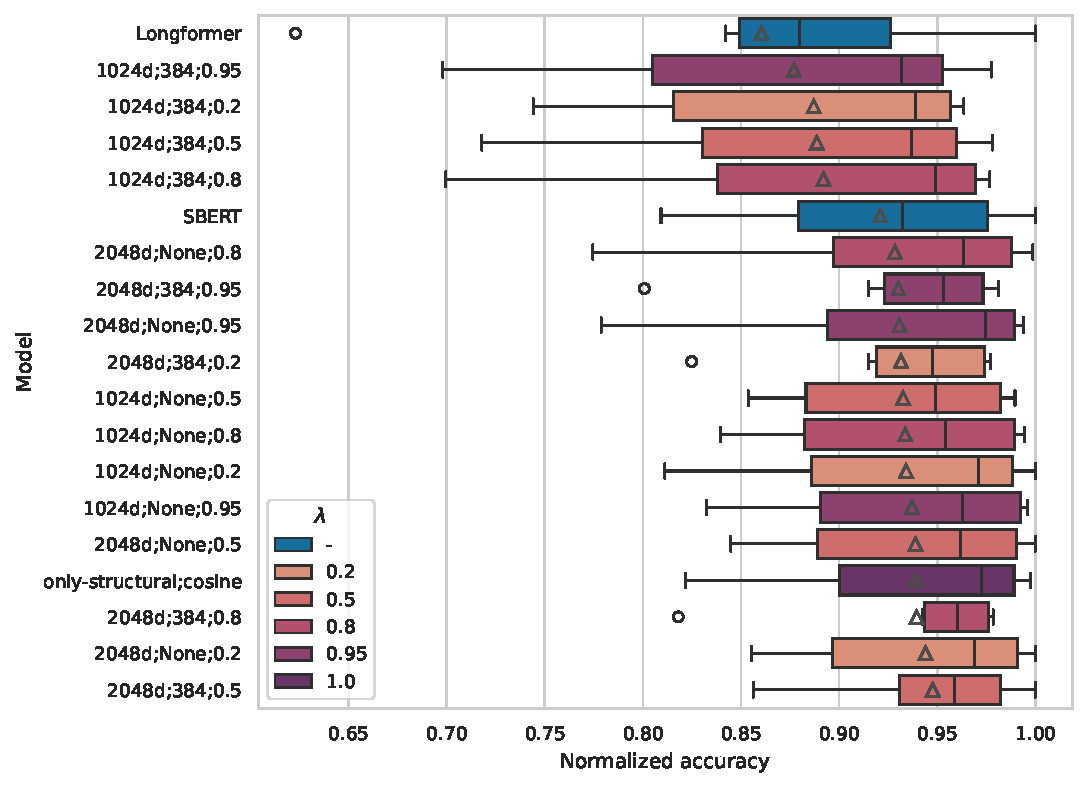
\includegraphics[width=0.85\textwidth]{img/cos_weighting.pdf}

  \caption{Performances of all weighting variants trained with cosine
  structural loss. We compare the student models to Longformer, SBERT and
  \Model{only-structural;cosine}.}

  \label{fig:cos_weighting}

\end{figure}

We highlight the difference in performance between \Model{None;$\lambda$=0.5}
and \Model{no-weighting}. These models' losses are exactly the same, except
that the gradients in \Model{None;$\lambda$=0.5} are halved. This results in a
noticeable drop in performance. However, even with the gradients being halved,
\Model{384;$\lambda$=0.5} beats \Model{no-weighting} variant. This further
emphasizes the importance of masking-out structural loss for long inputs.

\subsubsection{Weighting a contextual and the max-marginals MSE structural
loss}

As we ascertain in Section~\ref{section:projections_mm_mse}, with max-marginals
MSE structural loss, the projections that perform the best are
\Proj{S:768(ReLU)x1024(ReLU)x768;C:768} with \Model{DM;100d} contextual
teacher. However, even with this projection and contextual teacher, the model
performs worse than \Model{only-structural;mm-MSE}. Nevertheless, we continue
experimenting with the given projections and contextual teacher to see, if we
can improve the model by different weightings of the contextual and
max-marginals MSE structural losses and perhaps show that with smaller
contextual weight, the model may benefit from the contextual loss.

Again we compare the weighting variants to Longformer, SBERT, \Model{DM;100d},
and \Model{only-structural;mm-MSE}. We display the models' performances in
Figure~\ref{fig:mm_mse_weighting}. In the case of max-marginals MSE, masking
out structural loss for some inputs has significant negative effects on the
performance. As the loss is masked for some inputs, the number of negatives for
each input effectively decreases. As we discuss in
Section~\ref{section:composite_analysis}, max-marginals MSE causes the model to
place embeddings of different inputs further apart in the embedding space. With
less negatives, the model may move an embedding actually closer to a different
embedding, which however has been masked out. Note that the weighting variants
with higher $\lambda$ suffer from this effect considerably more.

Even without any masking, the different losses weightings fail to improve the
score of \Model{only-structural;mm-MSE}. When comparing the two nearly
identical weighting variants \Model{no-weighting} and
\Model{None;$\lambda$=0.5}, we see that \Model{no-weighting}, which trains
with gradients twice as big, is worse. This suggests that, with the
max-marginals MSE structural loss, the more we train with the contextual loss,
the worse is the model going to be. Ultimately this confirms the conclusions
from Section~\ref{section:projections_mm_mse}, where we do not find any
projections with which would the model benefit from a contextual loss.

\begin{figure}

  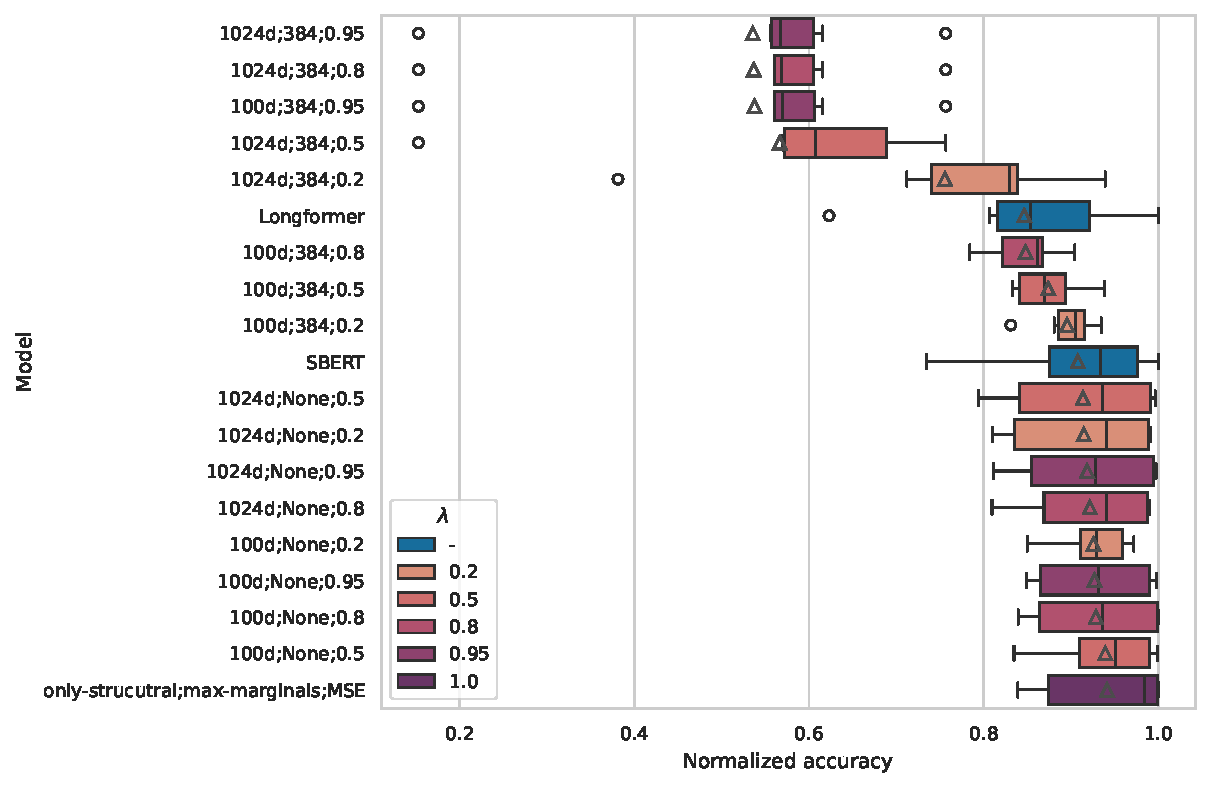
\includegraphics[width=0.9\textwidth]{img/mm_mse_weighting.pdf}

  \caption{Performances of all weighting variants for max-marginals MSE
  structural loss. We compare the students to Longformer, SBERT,
  \Model{DM;100d} contextual teacher and \Model{only-structural;mm-MSE}.}

  \label{fig:mm_mse_weighting}

\end{figure}

\section{Summary}\label{section:experiments_summary}

After an extensive experimentation with our teacher-student training method, we
summarize what we test, but mainly how we interpret the results and what
conclusions we draw from them.

First, in Section~\ref{section:structural_loss}, we experiment with simple and
composite structural losses. While simple losses focus only on the similarity
between the student's and the corresponding teacher's embedding, composite
losses also take advantage of the in-batch teacher's embedding of different
inputs. We find that the best performing simple structural loss is cosine,
which is able to surpass even SBERT. This shows that the combination of
Longformer's architecture, notably its longer maximum context, and distillation
of SBERT's embeddings can boost the student's performance even above the level
of the structural teacher. However, cosine is easily surpassed by the best
performing composite loss, which is max-marginals with MSE. As we show in
Section~\ref{section:composite_analysis}, max-marginals MSE losses use SBERT's
embeddings to increase the distance between student's embeddings of distinct
inputs. This shows that distillation of a certain quality from a student model,
may be less effective than just increasing the difference between distinct
inputs' embeddings.

In Section~\ref{section:structural_and_contextual}, we try to leverage the
contextual loss to improve the models trained with just the cosine or
max-marginals MSE structural loss. After finding promising training
hyperparameters for Paragraph Vector, we show that the contextual loss alone
can improve Longformer's results, yet it cannot surpass SBERT or the student
models trained with just the structural loss. This demonstrates that in our
setting, the contextual teacher is more important to the student's performance
than the contextual teacher. We also find the optimal contextual loss for
cosine and max-marginals MSE loss. In case of cosine structural loss, we see
that the student can benefit from both the contextual and the structural loss,
if the contextual loss is less exact and gives the student enough freedom. With
the max-marginals MSE structural loss, the contextual loss needs to be far less
strict and even then it fails to improve the student model trained with just
the structural loss. We also try a more involved ways to weight the contextual
and the structural loss. In the case of max-marginals MSE structural loss, we
find that even with a large emphasis on the structural loss, the student model
suffers from both the contextual loss and the max-marginals MSE loss used at
the same time. And so, we conclude that max-marginals MSE is incompatible with
our training method. On the other hand, with cosine structural loss the student
model behaves intuitively. The student model prefers an equal balance of the
structural and the contextual loss, where the structural loss is used only for
inputs which the structural teacher can encode whole.
